\chapter{Background}
% SE PÅ SamuelsenS MASTEROPPGAVE FOR INSPIRASJON (TROR HAN CLUSTERA OG KLASSIFISERTE HOVEDKONSEPTENE HAN BYGDE PÅ).
Kulepunkter \tcol[gray]{(bulletpoints)} fra mulige inspirasjoner og referanser \tcol[gray]{(pga. "Write a few lines summarizing relevant articles one comes across (which one is likely to refer to in the final report)" — Jims master-skrivingsdokument)}.



% SECTION 1

\section{Taking inspiration from psychology}






% SECTION 2

\section{Taking inspiration from natural phenomena}
The intriguing, diverse, and complex phenomena of nature have for long served as exciting inspirations to human engineers and researchers [ant-colonies, boids, swarms, beeclust]. One other such phenomena, studied and modelled, is the synchronously firing fireflies in forests, as can be seen an example of in Figure \ref{fig:synched_fireflies_phenomenon}.

\begin{figure}[!ht]
	\centering
	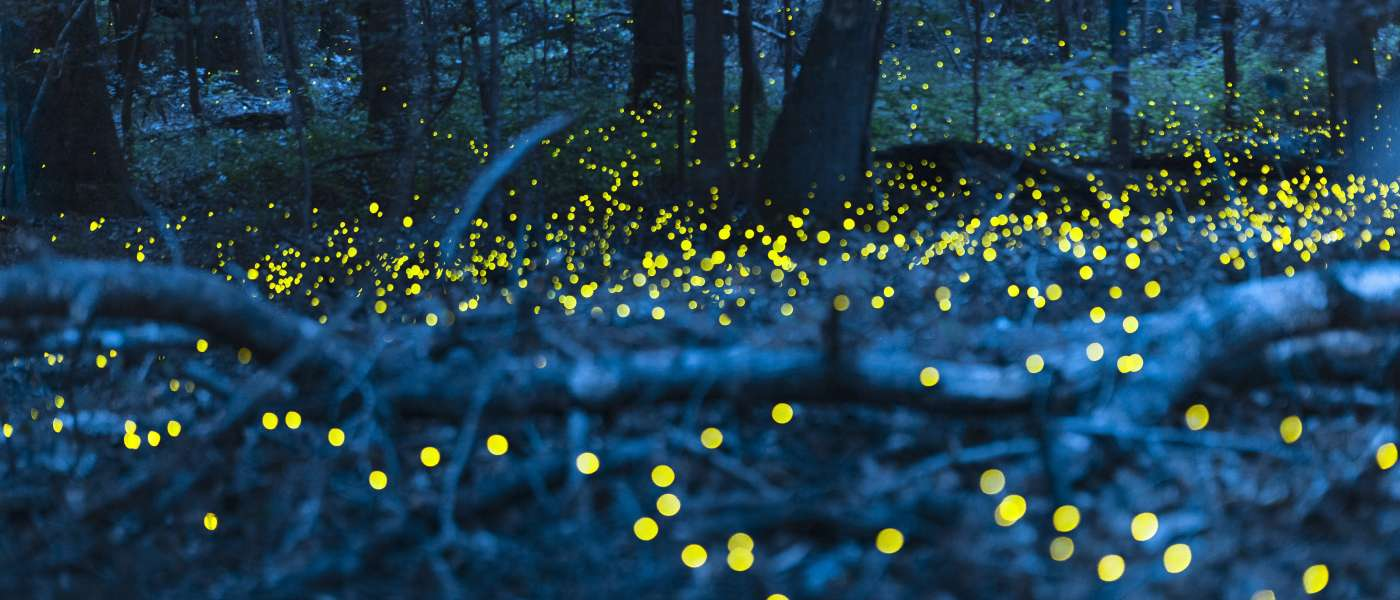
\includegraphics[width=0.9\linewidth]{Assets/Figures/synchronized_fireflies_phenomenon.jpg}
	\caption{Synchronous fireflies at Congaree National Park, United States \cite{synched_fireflies_phenomenon}.}
	\label{fig:synched_fireflies_phenomenon}
\end{figure}

This phenomenon of fireflies synchronizing to each other has inspired scientists like Mirollo \& Strogatz \cite{mirollo_strogatz_PCO_synch} and in later time Kristian Nymoen et al. \cite{nymoen_synch}, to model and replicate this natural phenomenon in human-engineered systems. It turns out that this is not a biological, but mathematical, problem. Given the periodic and repeating nature of the flashing/firing of the fireflies, modelling a firefly has been done by looking at each firefly as a periodic signal or oscillator. This work \cite{mirollo_strogatz_PCO_synch, nymoen_synch} then ties into the broader work on synchronizing oscillators which has been subject to study for some time now []. What separates Mirollo-Strogatz and K. Nymoen's approaches from these other and previous oscillator-synchronizing methods, is mainly that here the oscillators are \textit{pulse-coupled} (which the fireflies also can be said to be), as opposed to the more ``standard'' and constraining \textit{phase-coupled} oscillators.



% SECTION 3

\section{Oscillators and oscillator-synchronization}

	\gjor{Beskriv dette så godt at du kan snakke fritt om oscillatorers \textbf{faser} og \textbf{frekvenser} senere (i Implementation f.eks.), spesielt i tilfelle for noen ikke har vært borti det før, eller tatt et Signalbehandlings-kurs}
	
	\gjor{Skill på Pulse-coupled Oscillators, og Phase-coupled Oscillators}
	
	Much of the terminology from \cite{nymoen_synch} is used here. An oscillator $i$ is characterized by its \textit{phase} $\phi_i(t)$, which is—at the start of its periodic signal period—initialized to 0 and evolves towards 1 at a rate of $\frac{d \phi_i(t)}{d t}$ — which is also called the \textit{frequency} of the oscillator. When oscillator $i$'s phase is equal to 1 (i.e. when $\phi_i(t)=1$, or when the periodic signal period is over), we say oscillator $i$ has \textit{phase-climaxed}.
	
	\subsection{Phase-adjustment}
				
	(If relevant and wanted) \nl
	Previous approaches to Phase-synchronization in oscillators (pulse- and/or phase-coupled).
		
	\subsection{Frequency-adjustment}
	
	(If relevant and wanted) \nl
	Previous approaches to Frequency-synchronization in oscillators (pulse- and/or phase-coupled) [fixed\_freqs, fixed\_range\_freqs] where the oscillators's frequencies are either equal and fixed, or where frequencies are bound to initialize and stay within a fixed interval/range.